\documentclass{scrartcl}			% defines the kind of document you want to produce

% Include different packages:
\usepackage[utf8x]{inputenc}
\usepackage[T1]{fontenc}
\usepackage{lmodern}
\usepackage[english]{babel}
\usepackage{amsmath}
\usepackage{graphicx}           	% include graphics
\usepackage{caption}	
\usepackage{subcaption}	 
\usepackage{hyperref}
\usepackage{epstopdf}
\usepackage{siunitx}
\usepackage{float}

\title{Neuroprothetics Exercise 7\\Filter Banks}
\author{ Laura Bielenberg }
\date{28. Juni 2019}

\begin{document} 					% Document begins here

\maketitle

\section{Tonotopy of a simplified cochlear implant model}

\subsection{Electrode center frequencies}
\begin{figure}[H]
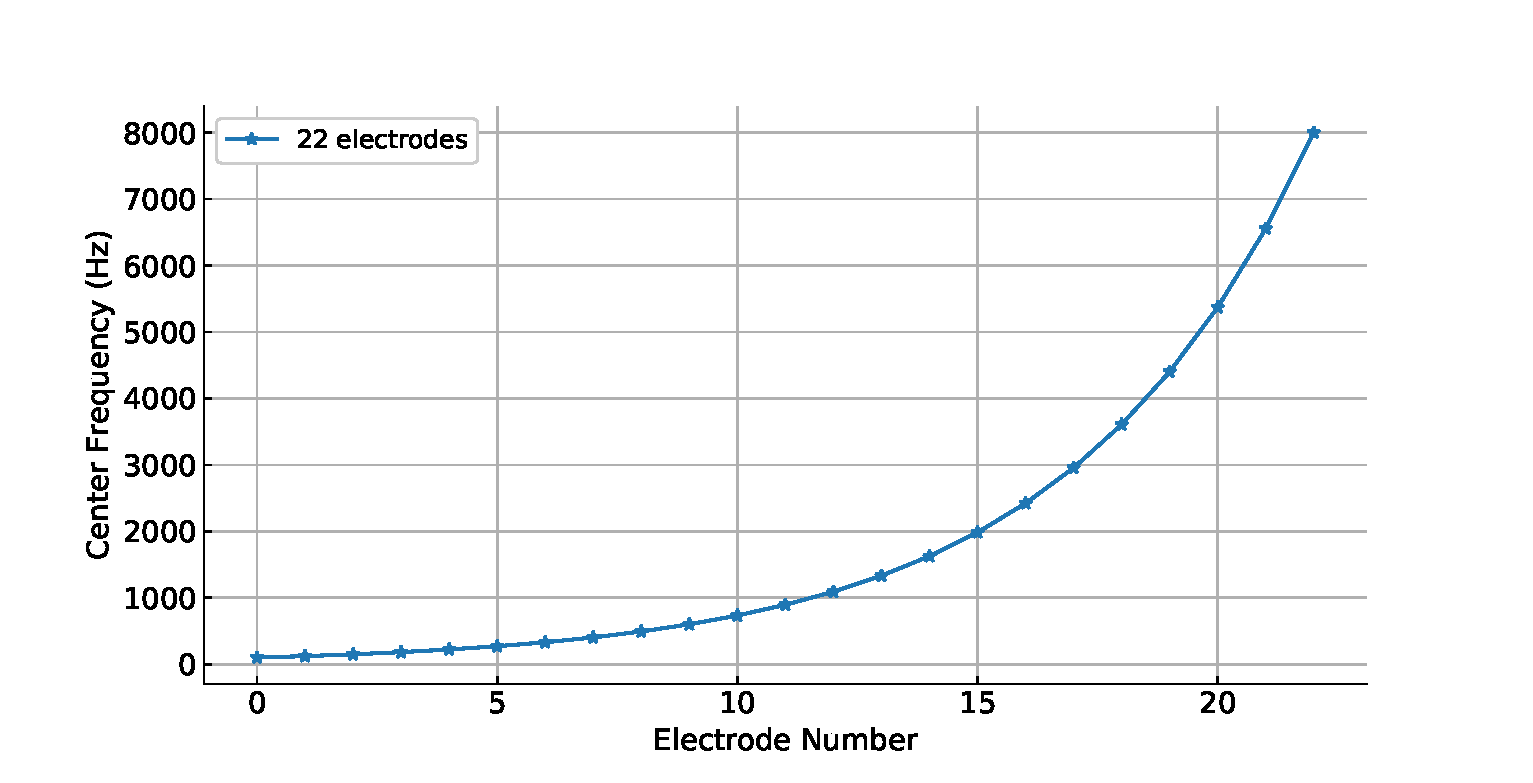
\includegraphics[width=\linewidth]{imgs/center_frequencies_22.eps}
    \caption{Center frequencies for CIs with different numbers of electrodes.} 
    \label{fig:center_freq} 
\end{figure}

%\begin{figure}[H]
%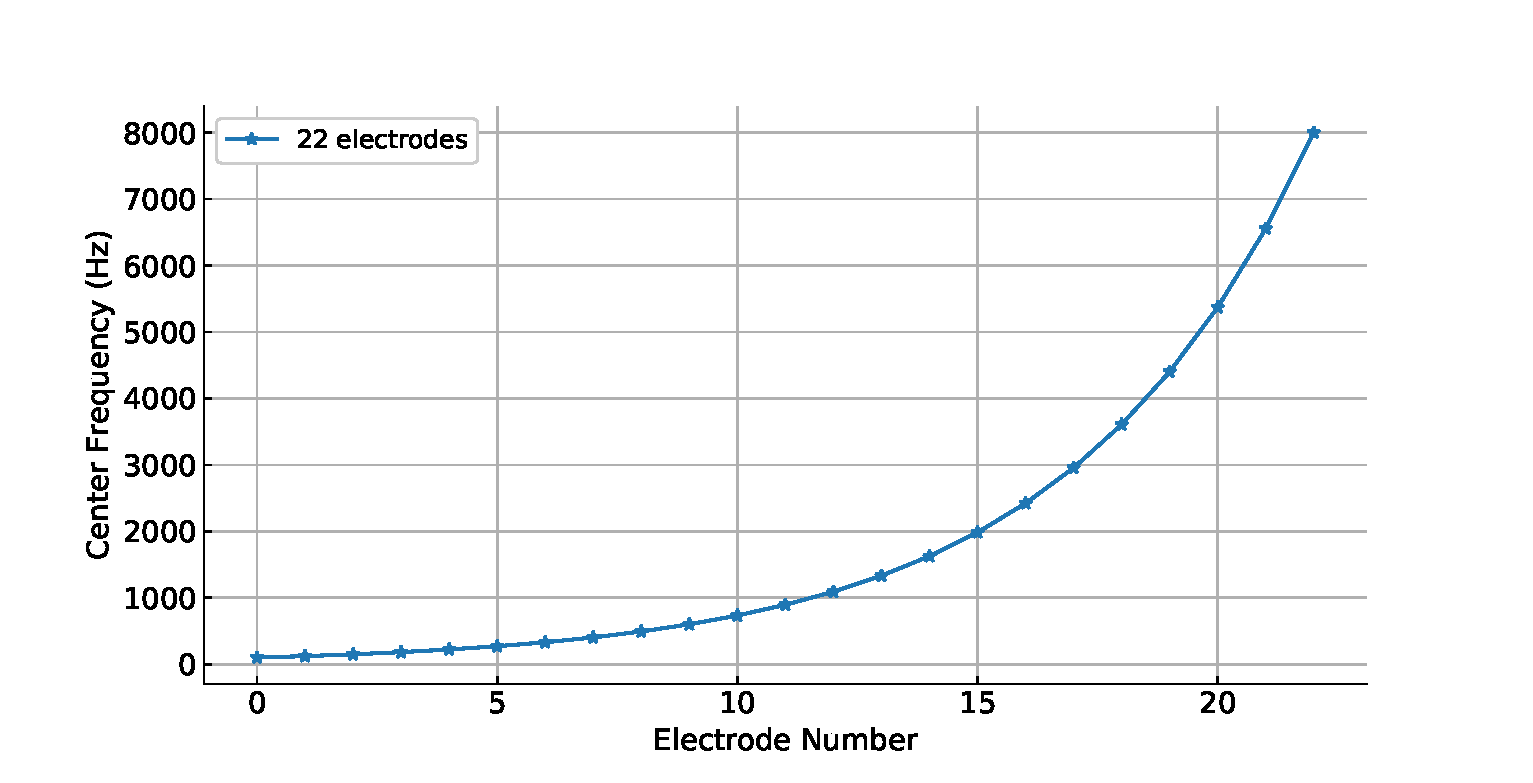
\includegraphics[width=\linewidth]{imgs/center_frequencies_22.eps}
%    \caption{} 
%    \label{fig:center_freq2} 
%\end{figure}

\subsection{Implement a filter bank}

\begin{figure}[H]
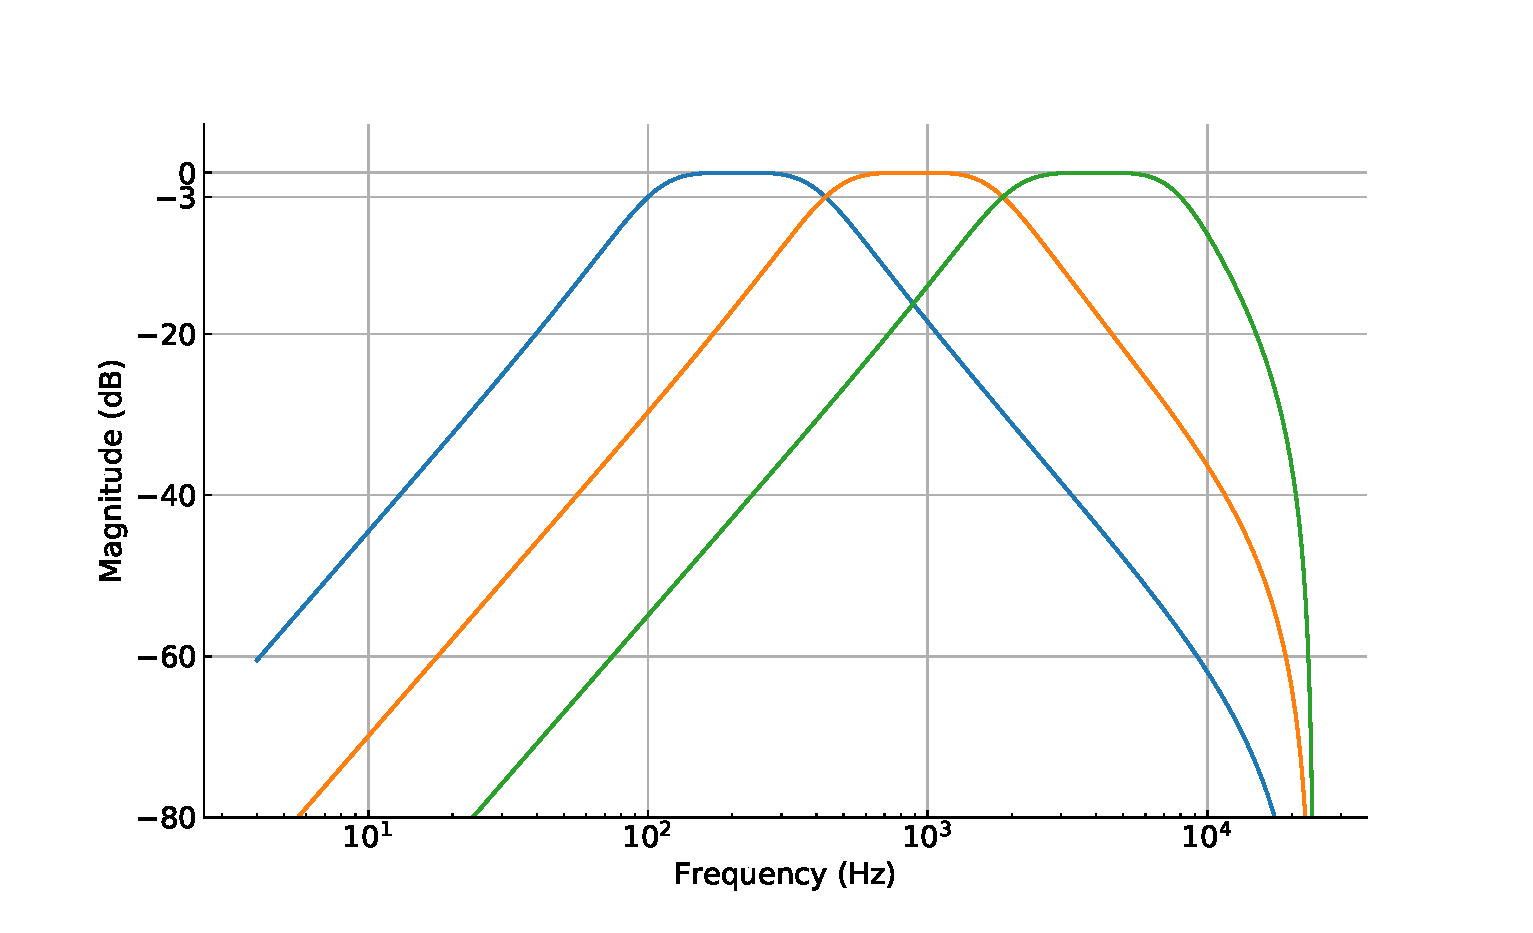
\includegraphics[width=\linewidth]{imgs/ci_with_3_electrodes.eps}
    \caption{Frequency response of a second-order  band-pass filter bank for a CI with three electrodes.} 
    \label{fig:ci_3} 
\end{figure}

\begin{figure}[H]
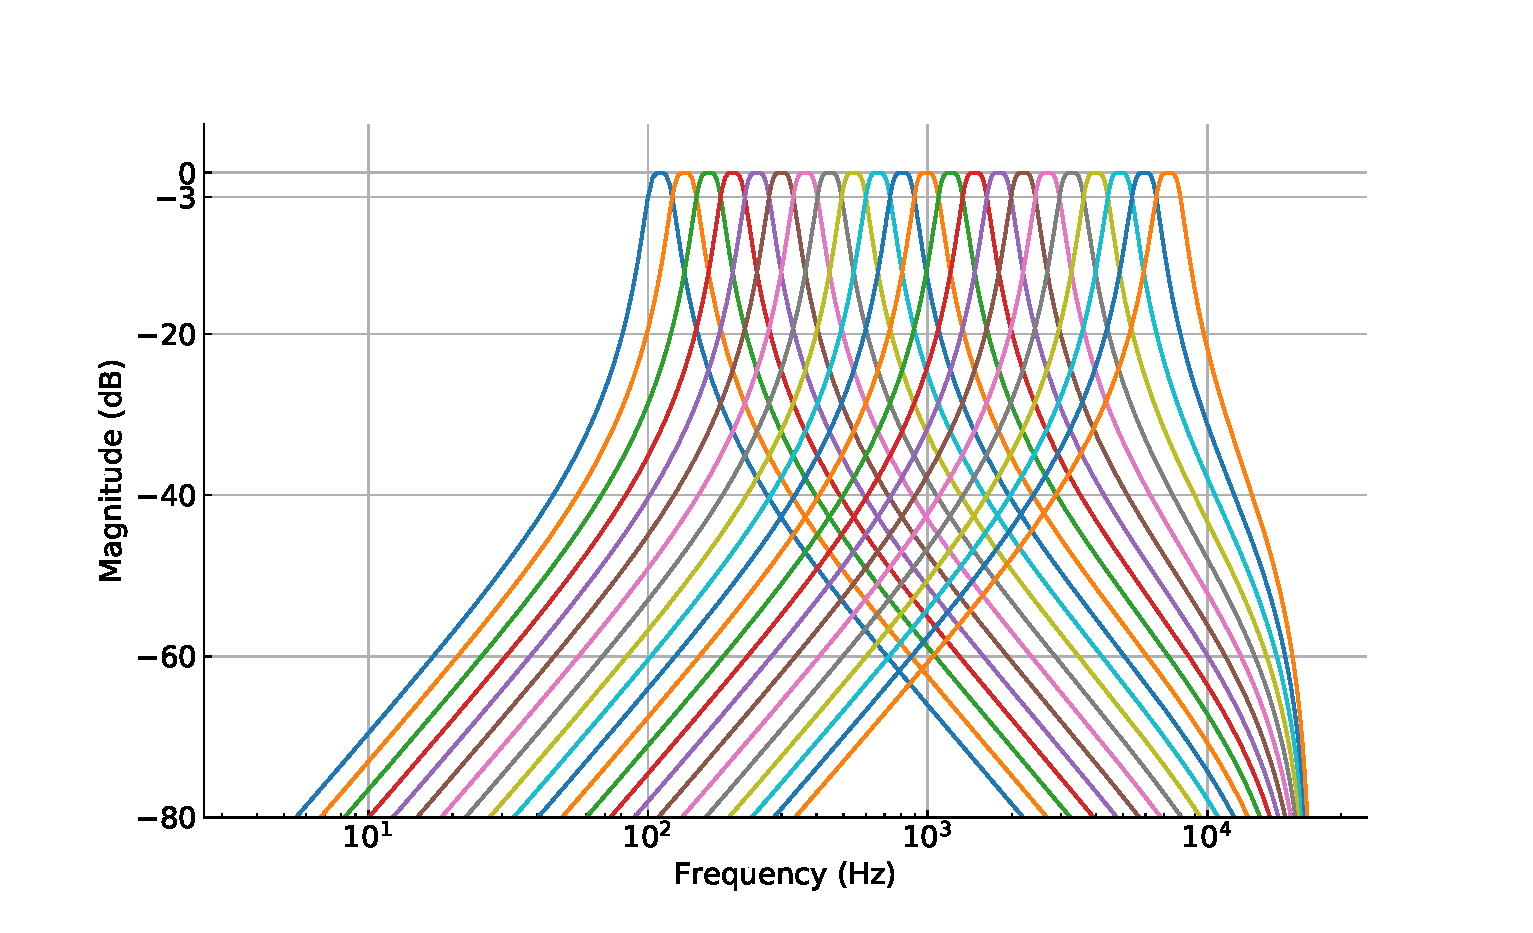
\includegraphics[width=\linewidth]{imgs/ci_with_22_electrodes.eps}
    \caption{Frequency response of a second-order  band-pass filter bank for a CI with 22 electrodes.} 
    \label{fig:ci_22} 
\end{figure}

\subsection{Filter a recorded signal}

\subsection{Join the channals}


\end{document}
